\chapter{Appendix}


%\section{Detailed Addition}

% Even sections are possible, but usually only used for several elements in, e.g.\ tables, images, etc.


% \section{Example 1}
% \cmark
% \section{Example 2}
% \xmark

% use tiny after centering
%\chapter{Tracking metrics overview}
\section{Tracking metrics overview}
\begin{table}[ht!]
\caption{Overview of popular tracking metrics}
\centering
\tiny
%\rotatebox{90}{
%\setlength{\extrarowheight}{5.5pt}
\renewcommand{\arraystretch}{2.5}
\begin{tabular}{|c|c|c|} 
\hline
\textbf{Metric}    & \textbf{Datasets/ Challenges}    & \textbf{Formula }                                                                                                                                                                                                                                                                                                                 \\ 
\hline
MOTA           & MOT Challenges    & $MOTA = \frac{|TP|-|FP|-|IDSWc|}{|GT|} $                                                                                                                                                                                                                                                                                  \\ 
\hline
IDF1           & MOT Challenges     & $IDF1 = \frac{|IDTP|}{|IDTP|+0.5|IDFN|+0.5|IDFP|}$                                                                                                                                                                                                                                                                        \\ 
\hline
HOTA           & MOT Challenges     & \begin{tabular}[c]{@{}l@{}}$DetA_{\alpha} = \frac{|TP|}{|TP|+|FN|+|FP|}$ \text{,    }    $AssA_{\alpha} = \frac{1}{|TP|}\sum_{c \in {TP}}A(c)$\\$A(c) = \frac{|TPA(c)|}{|TPA(c)|+|FNA(c)|+|FPA(c)|}$ \text{,    } $HOTA_{\alpha}=\sqrt{DetA_{\alpha}AssA_{\alpha}}$\end{tabular}                                                                       \\ 
\hline
MOTSA          & MOTS Challenge         & $MOTSA = \frac{|TP|-|FP|-|IDSWc|}{|GT|}$                                                                                                                                                                                                                                                                                  \\ 
\hline
sMOTSA         & MOTS Challenge    & \begin{tabular}[c]{@{}l@{}}$sMOTSA = \frac{\widetilde{TP} -|FP|-|IDSWc|}{|GT|}$\\$ \widetilde{TP} = \sum_{h \in TP} IoU(h, c(h))$\end{tabular}                                                                                                                                                                            \\ 
\hline
J              & DAVIS/YouTube-VOS   & \begin{tabular}[c]{@{}l@{}}$m(J,S) = \frac{1}{|O_S|}\sum_{o \in O_S} \frac{1}{|F_{S(O)}|}\sum_{f \in F_{s(o)}}J(m_o^f, g_o^f)$\\\end{tabular}                                                                                                                                                                             \\ 
\hline
F              & DAVIS/YouTube-VOS   & $m(F,S) = \frac{1}{|O_S|}\sum_{o \in O_S} \frac{1}{|F_{S(O)}|}\sum_{f \in F_{s(o)}}F(m_o^f, g_o^f)$                                                                                                                                                                                                                       \\ 
\hline
AP, AP50, AP75 & YouTube-VIS          &  \begin{tabular}[c]{@{}l@{}}$IoU(i,j) = \frac{\sum_{t=1}^T|m_t^i\cap m_t^j|}{\sum_{t=1}^T|m_t^i\cup m_t^j|}$\\$AP = mAP = \frac{1}{N}\sum_{i=1}^N AP_i$\end{tabular}                                                                                                                                                       \\ 
% \hline
% VPQ            &   Cityscapes-VPS      & \begin{tabular}{@{\labelitemi\hspace{\dimexpr\labelsep+0.5\tabcolsep}}l@{}}Probably very sensitive to id switches like J\end{tabular}                                                                                                     & $VPQ = \frac{1}{K} \sum_{k}\frac{1}{N_{classes}}\sum_{c}\frac{\sum_{(p,g) \in TP_{c}^k}IoU_{2D/3D}(p,g)}{|TP_c^k|+\frac{1}{2}|FP_c^k|+\frac{1}{2}|FN_c^k|}$                                                                                                                                                             \\ 
\hline
STQ            &  MOTChallenge-STEP   & \begin{tabular}[c]{@{}l@{}}$AQ = \frac{1}{|gt_tracks|}\sum_{g \in gt_tracks} \frac{1}{|gt_{id}(g)|} \sum_{p,|p \cap g| \neq \emptyset}TPA(p,g) x IoU_{id}(p,g)$\\$SQ = mIoU = \frac{1}{|C|}\sum_{c\in C}\frac{|pr_{sem}(c)\cap gt_{sem}(c)|}{|pr_{sem}(c)\cup gt_{sem}(c)|}$\\$STQ = (AQ x SQ)^{\frac{1}{2}}$\end{tabular}  \\
\hline
\end{tabular}
 \label{Tab:metrics}
%}
\end{table}

\clearpage

\section{Crowdness analysis encoders} \label{seq: appendix_croudness}

\begin{figure} [ht!]
    \centering
    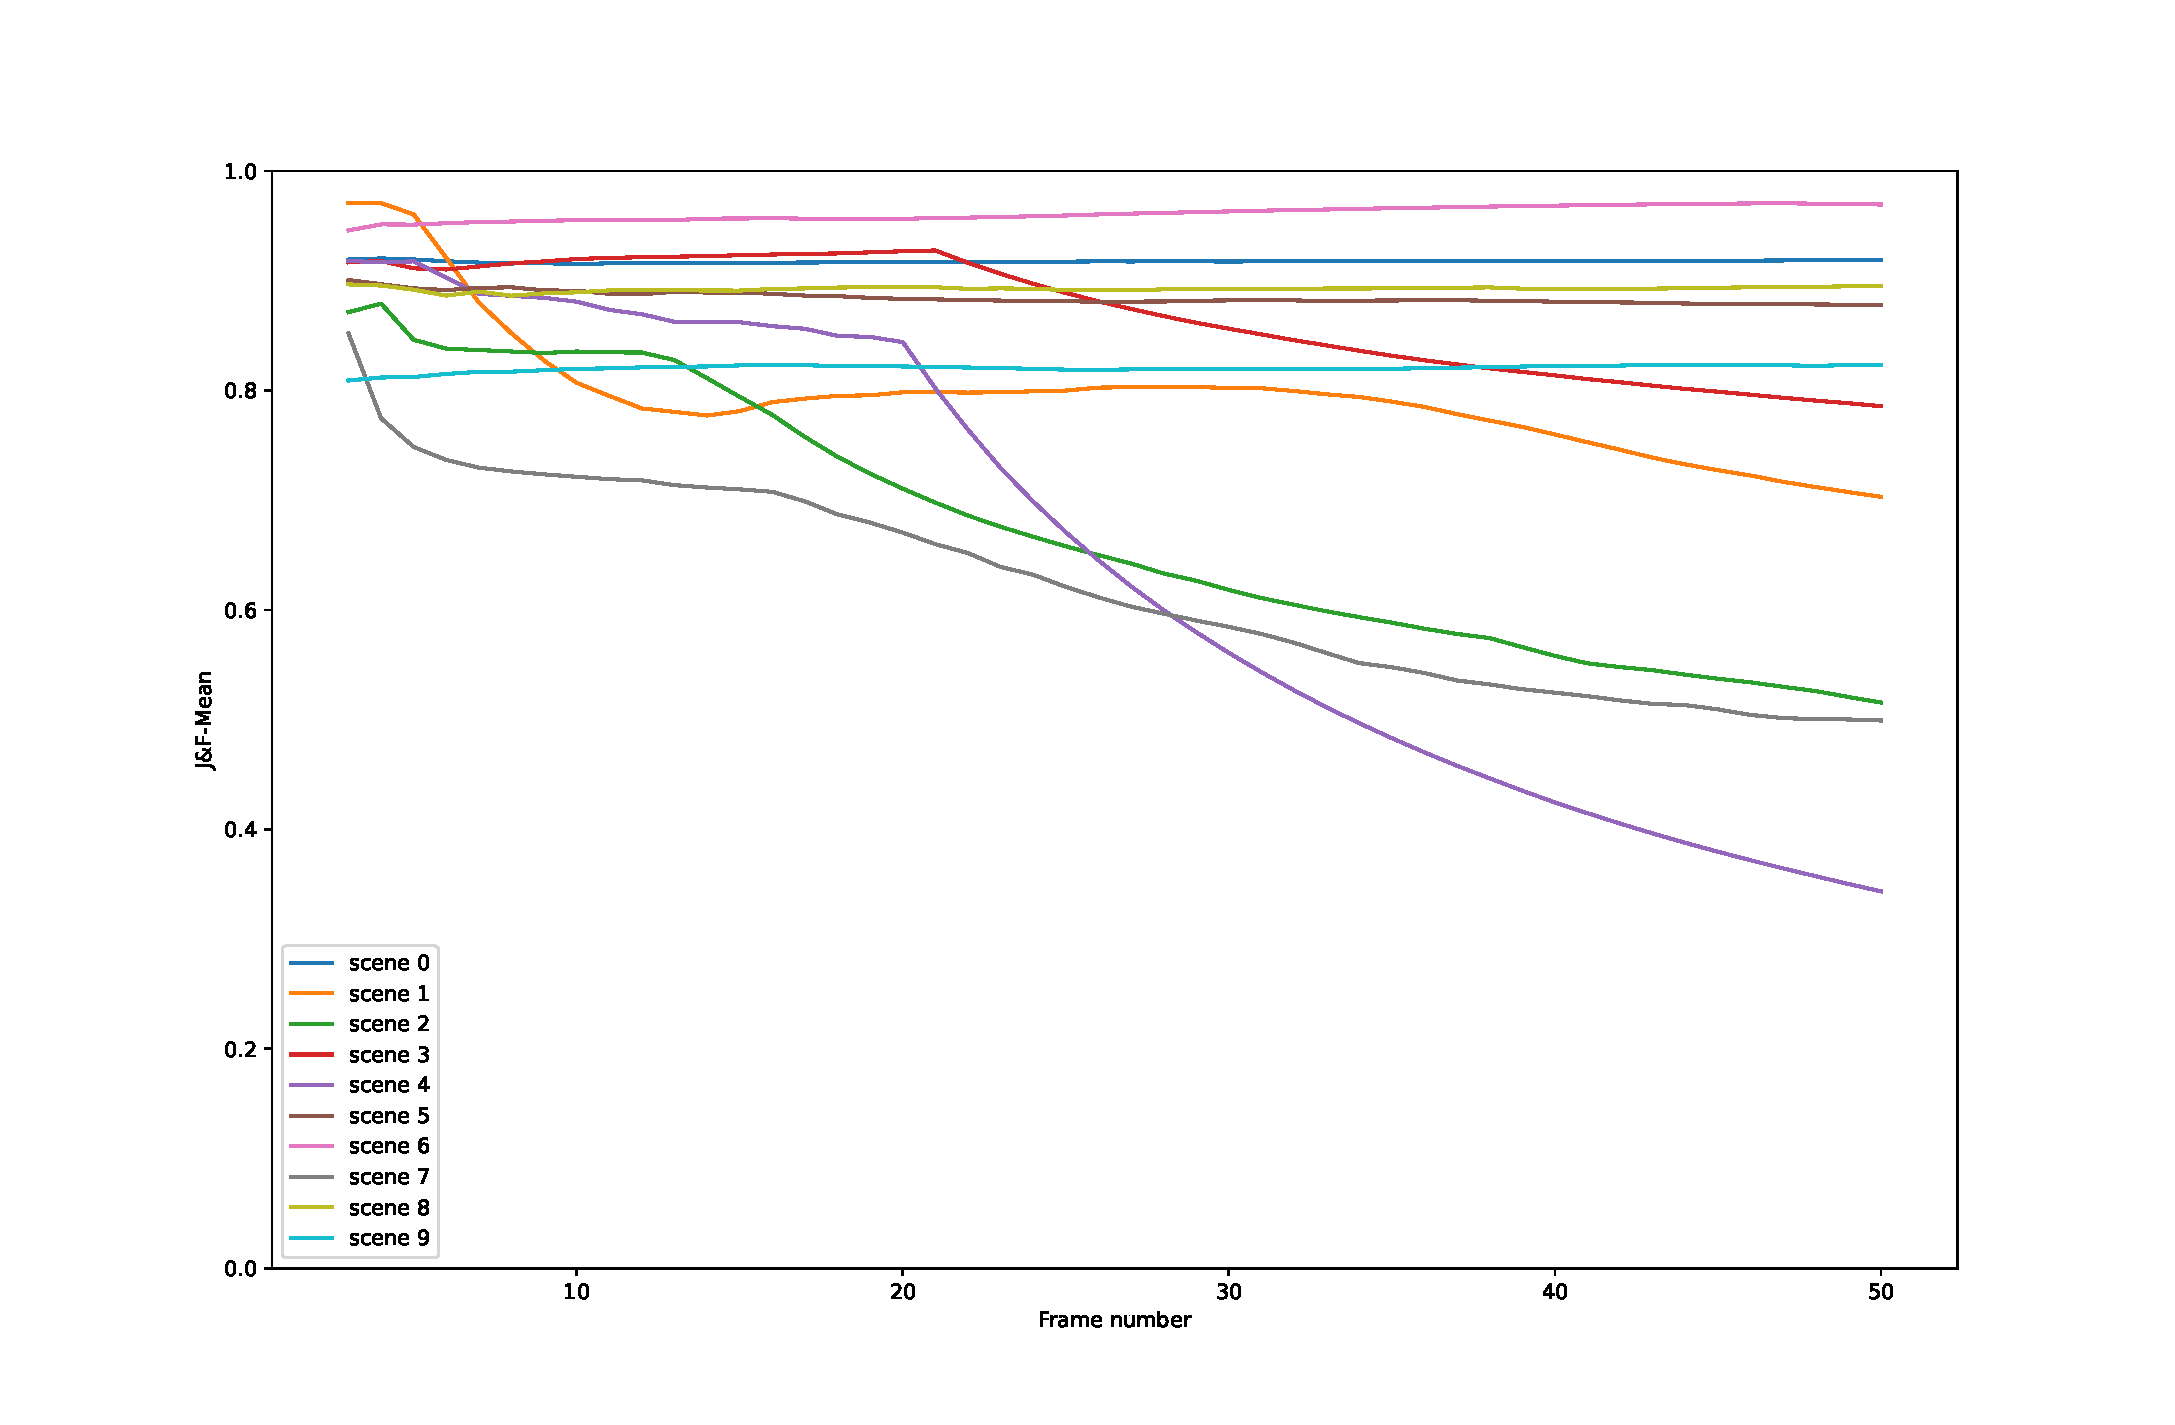
\includegraphics[trim={ 0 2cm 0 1.75cm},width=0.6\linewidth]{figures/appendix/9_backbone_att_fpn_fast_rotation-J_F.pdf}
    \caption{J\&F-Mean backbone encoder on all rotation fast sequences}
    \label{fig:backbone_j_f}
    
\end{figure}

\begin{figure} [ht!]
    \centering
    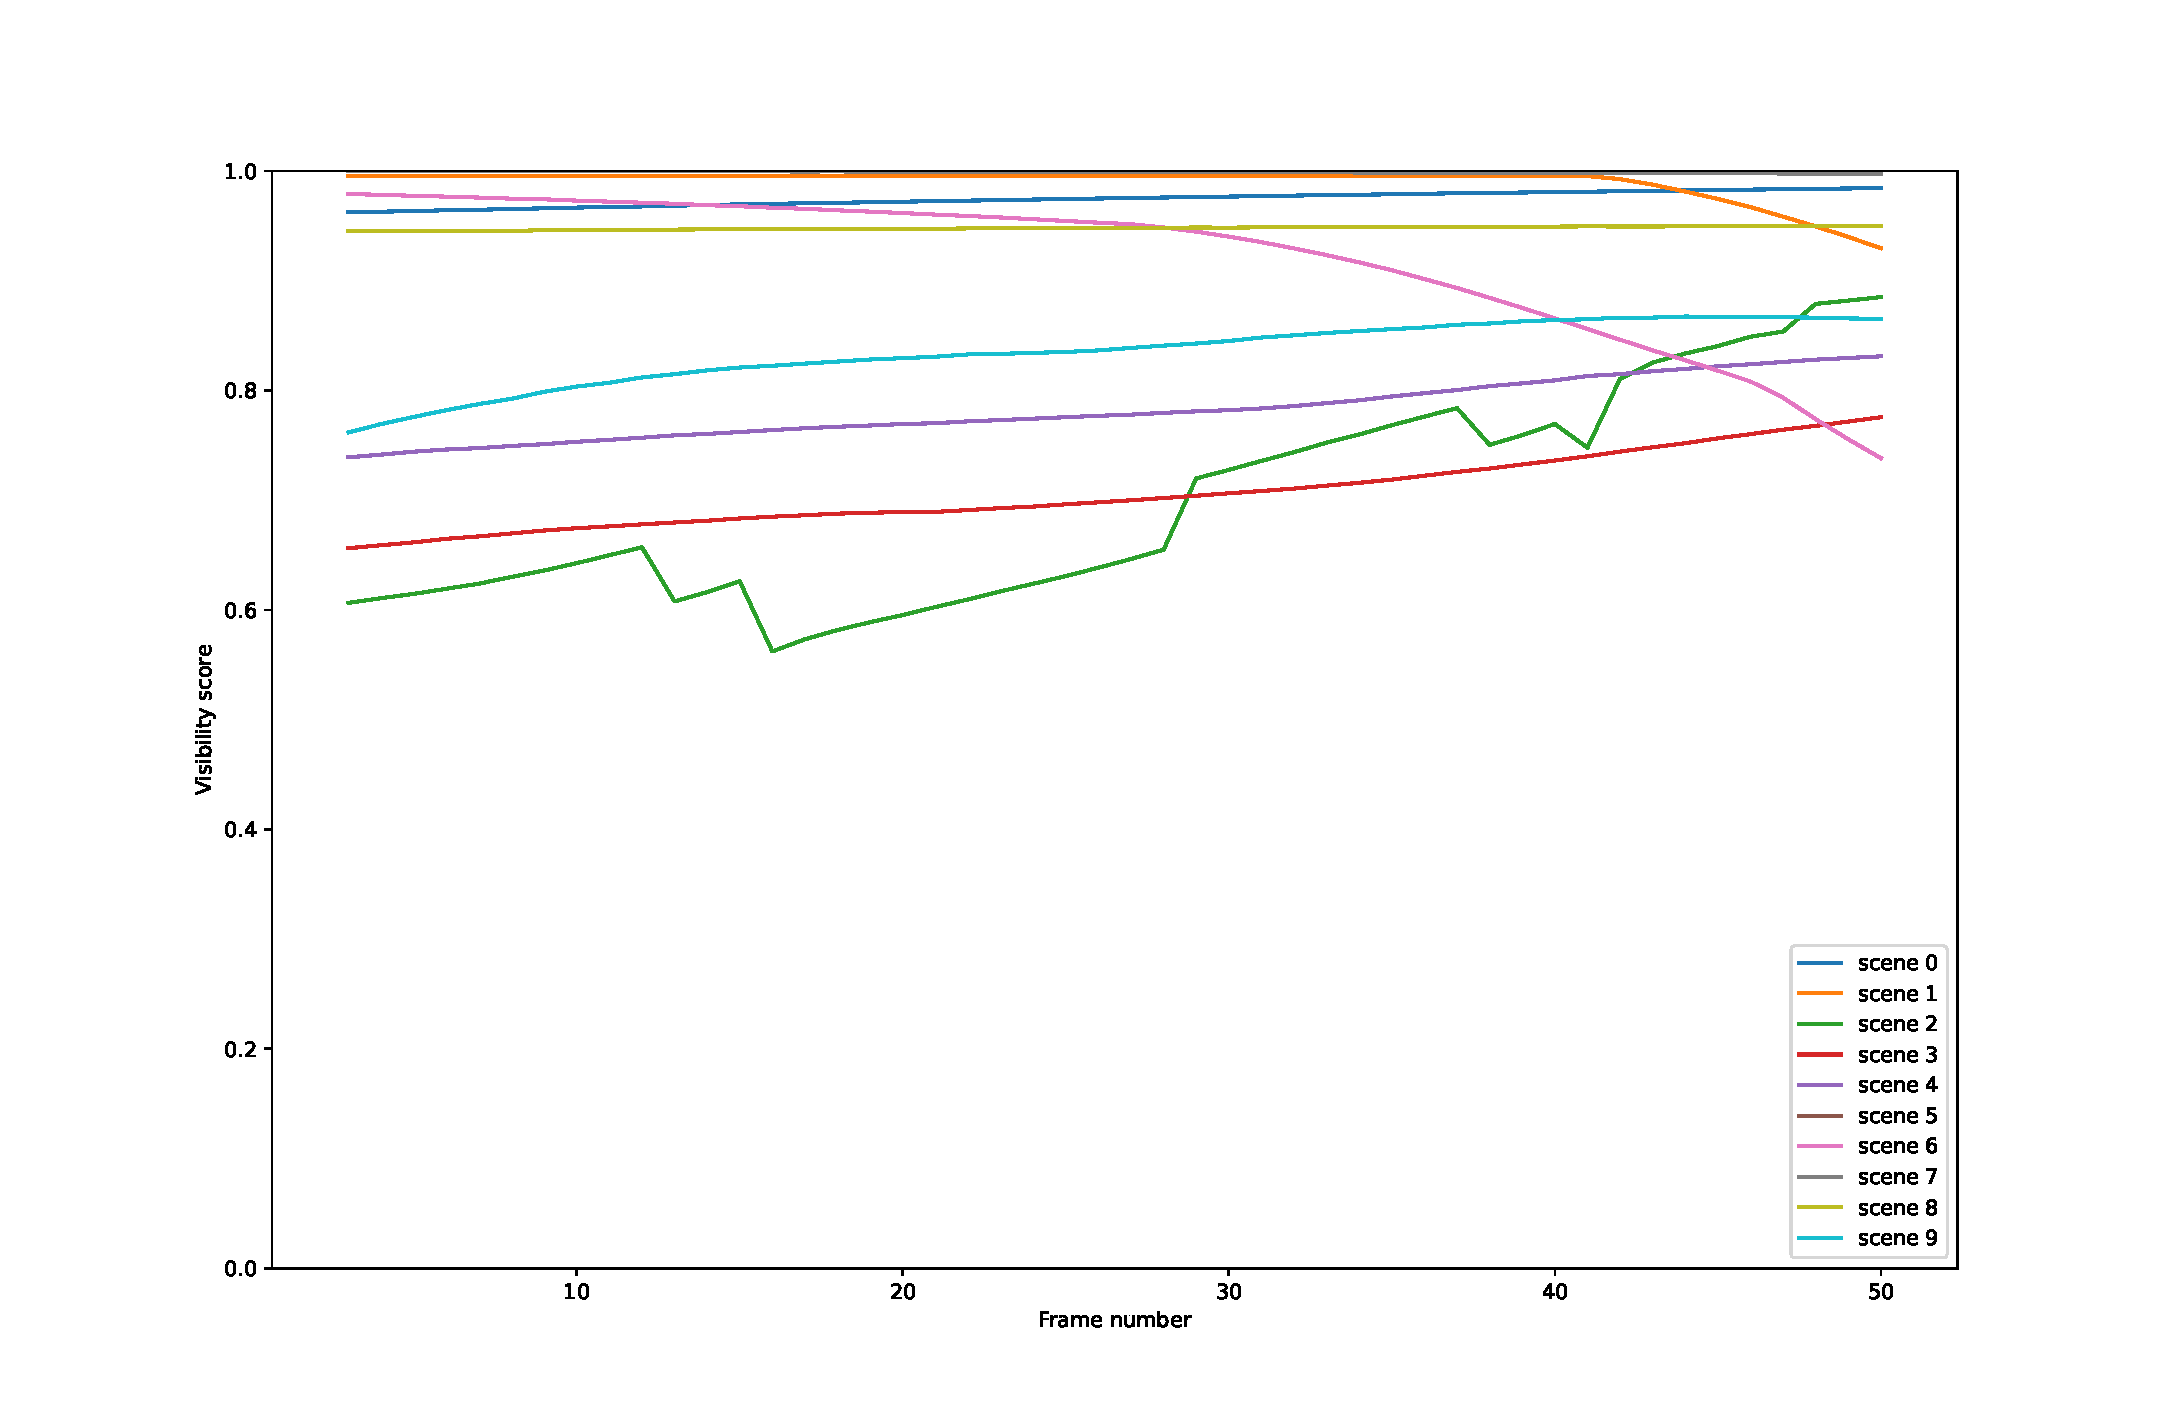
\includegraphics[trim={ 0 2cm 0 2.5cm},width=0.6\linewidth]{figures/appendix/9_backbone_att_fpn_fast_rotation-visibility.pdf}
    \caption{Visibility score backbone encoder on all rotation fast sequences}
    \label{fig:backbone_visibility}
    
\end{figure}
\begin{figure} [ht!]
    \centering
    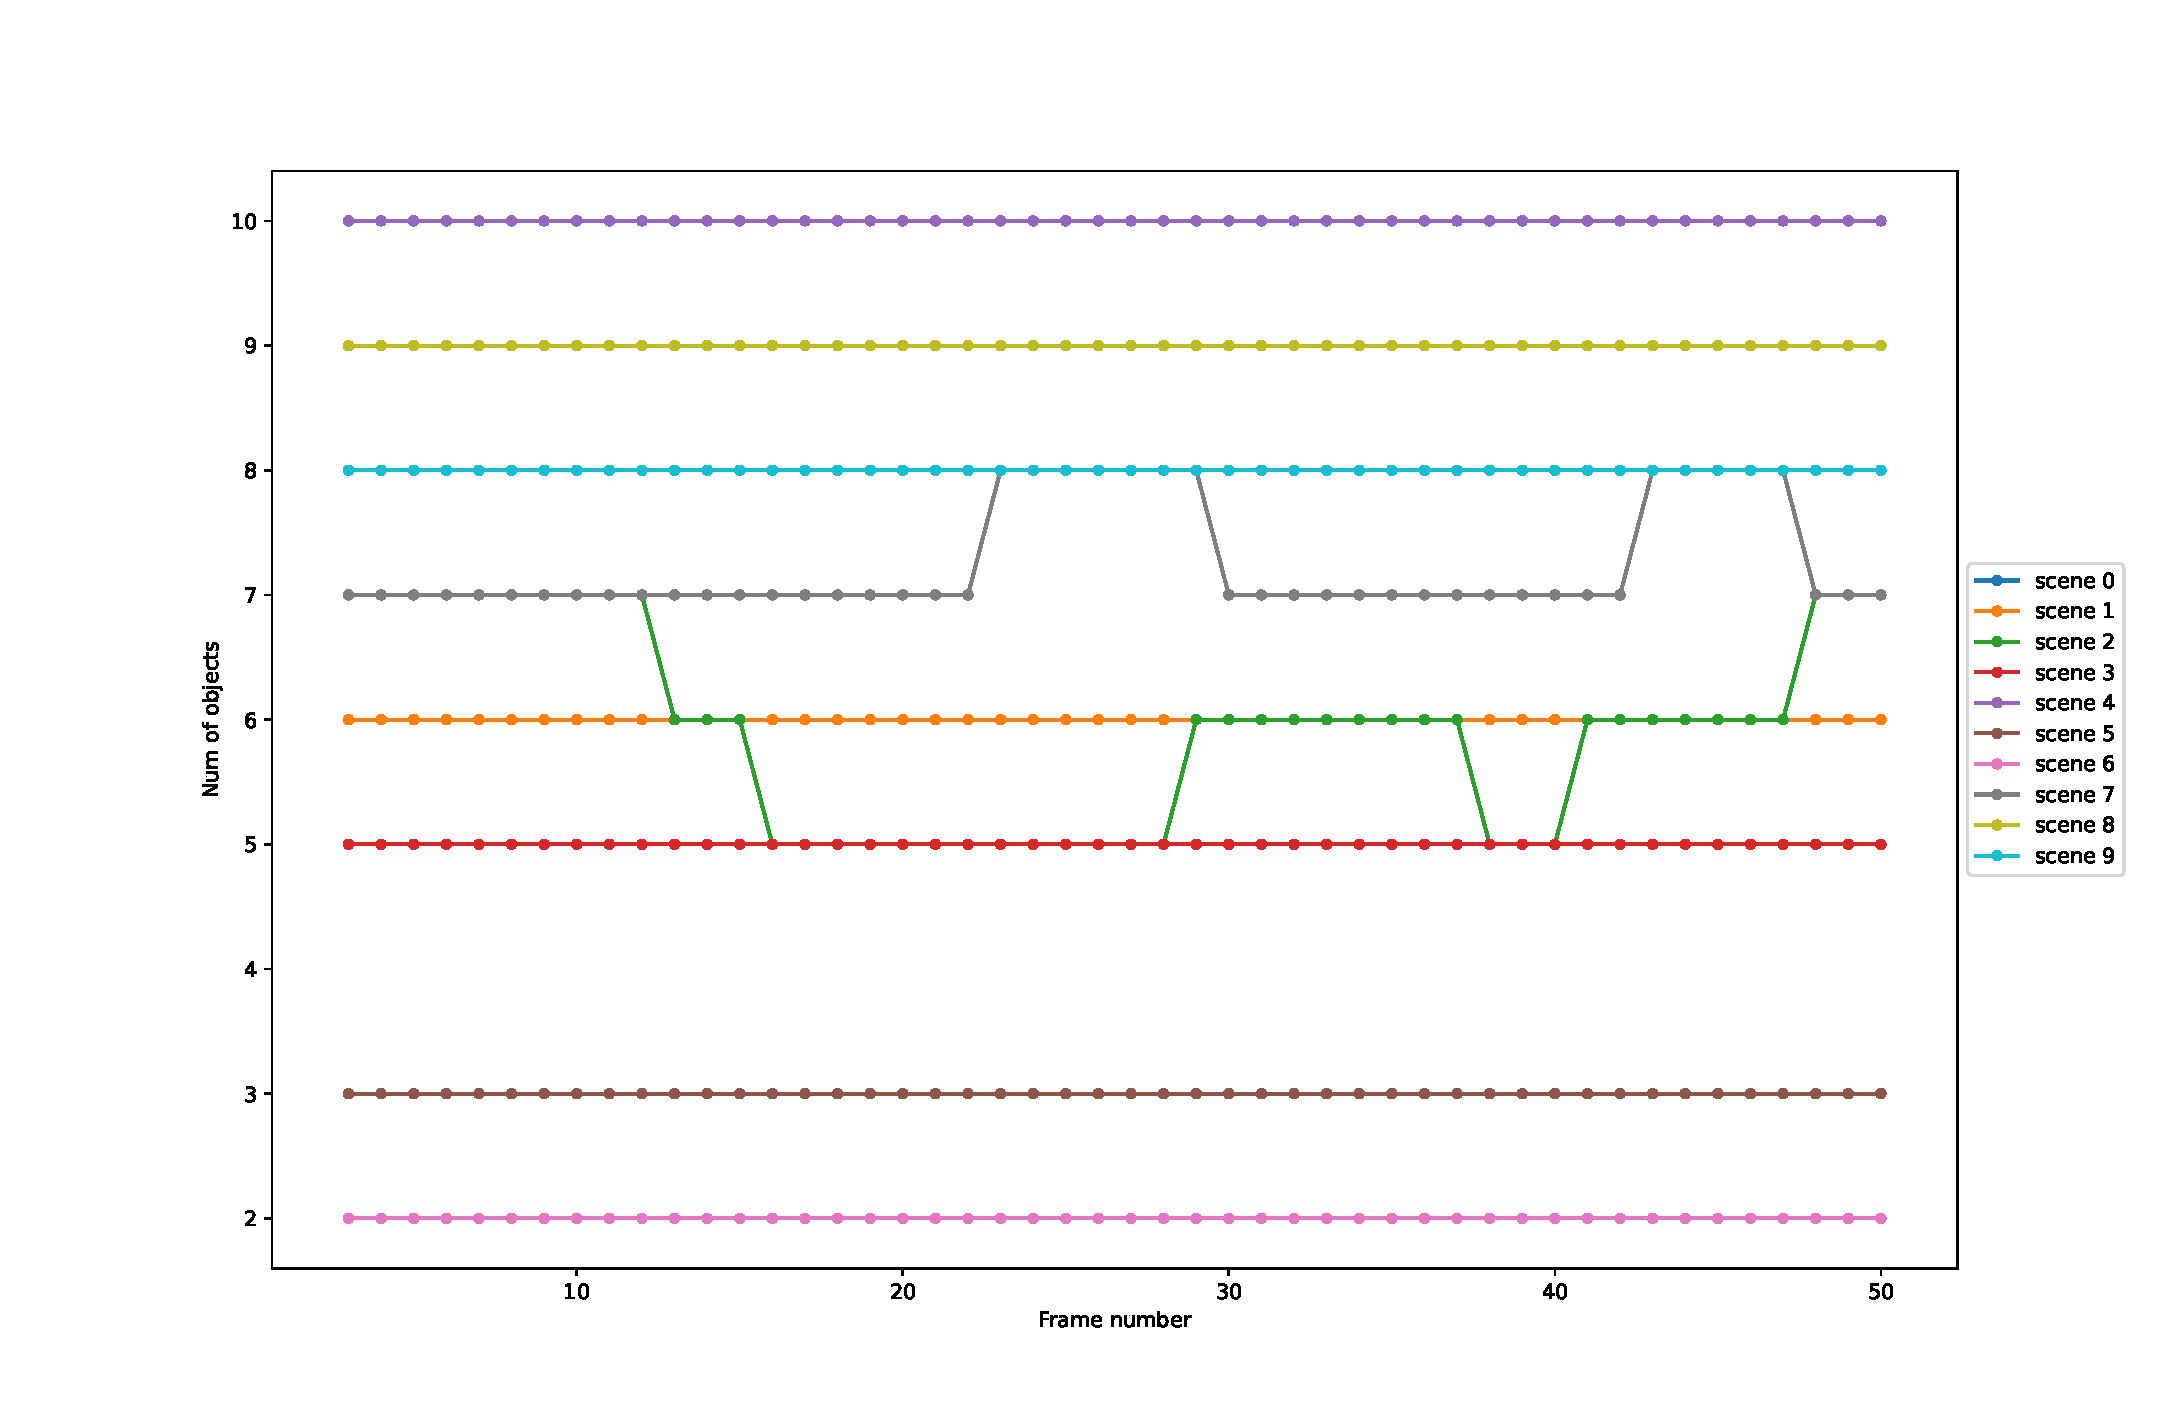
\includegraphics[trim={ 0 2cm 0 2.5cm},width=0.6\linewidth]{figures/appendix/9_backbone_att_fpn_fast_rotation-crowdness.pdf}
    \caption{Num. of objects backbone encoder on all rotation fast sequences}
    \label{fig:backbone_crowdness}
    
\end{figure}
%%%%%%%%%%%%%%%%bbox%%%%%%%%%%%%%%%%%%%%%%%%%%%%%%%%%%%%%%%%%%%%%%%
\begin{figure} [ht!]
    \centering
    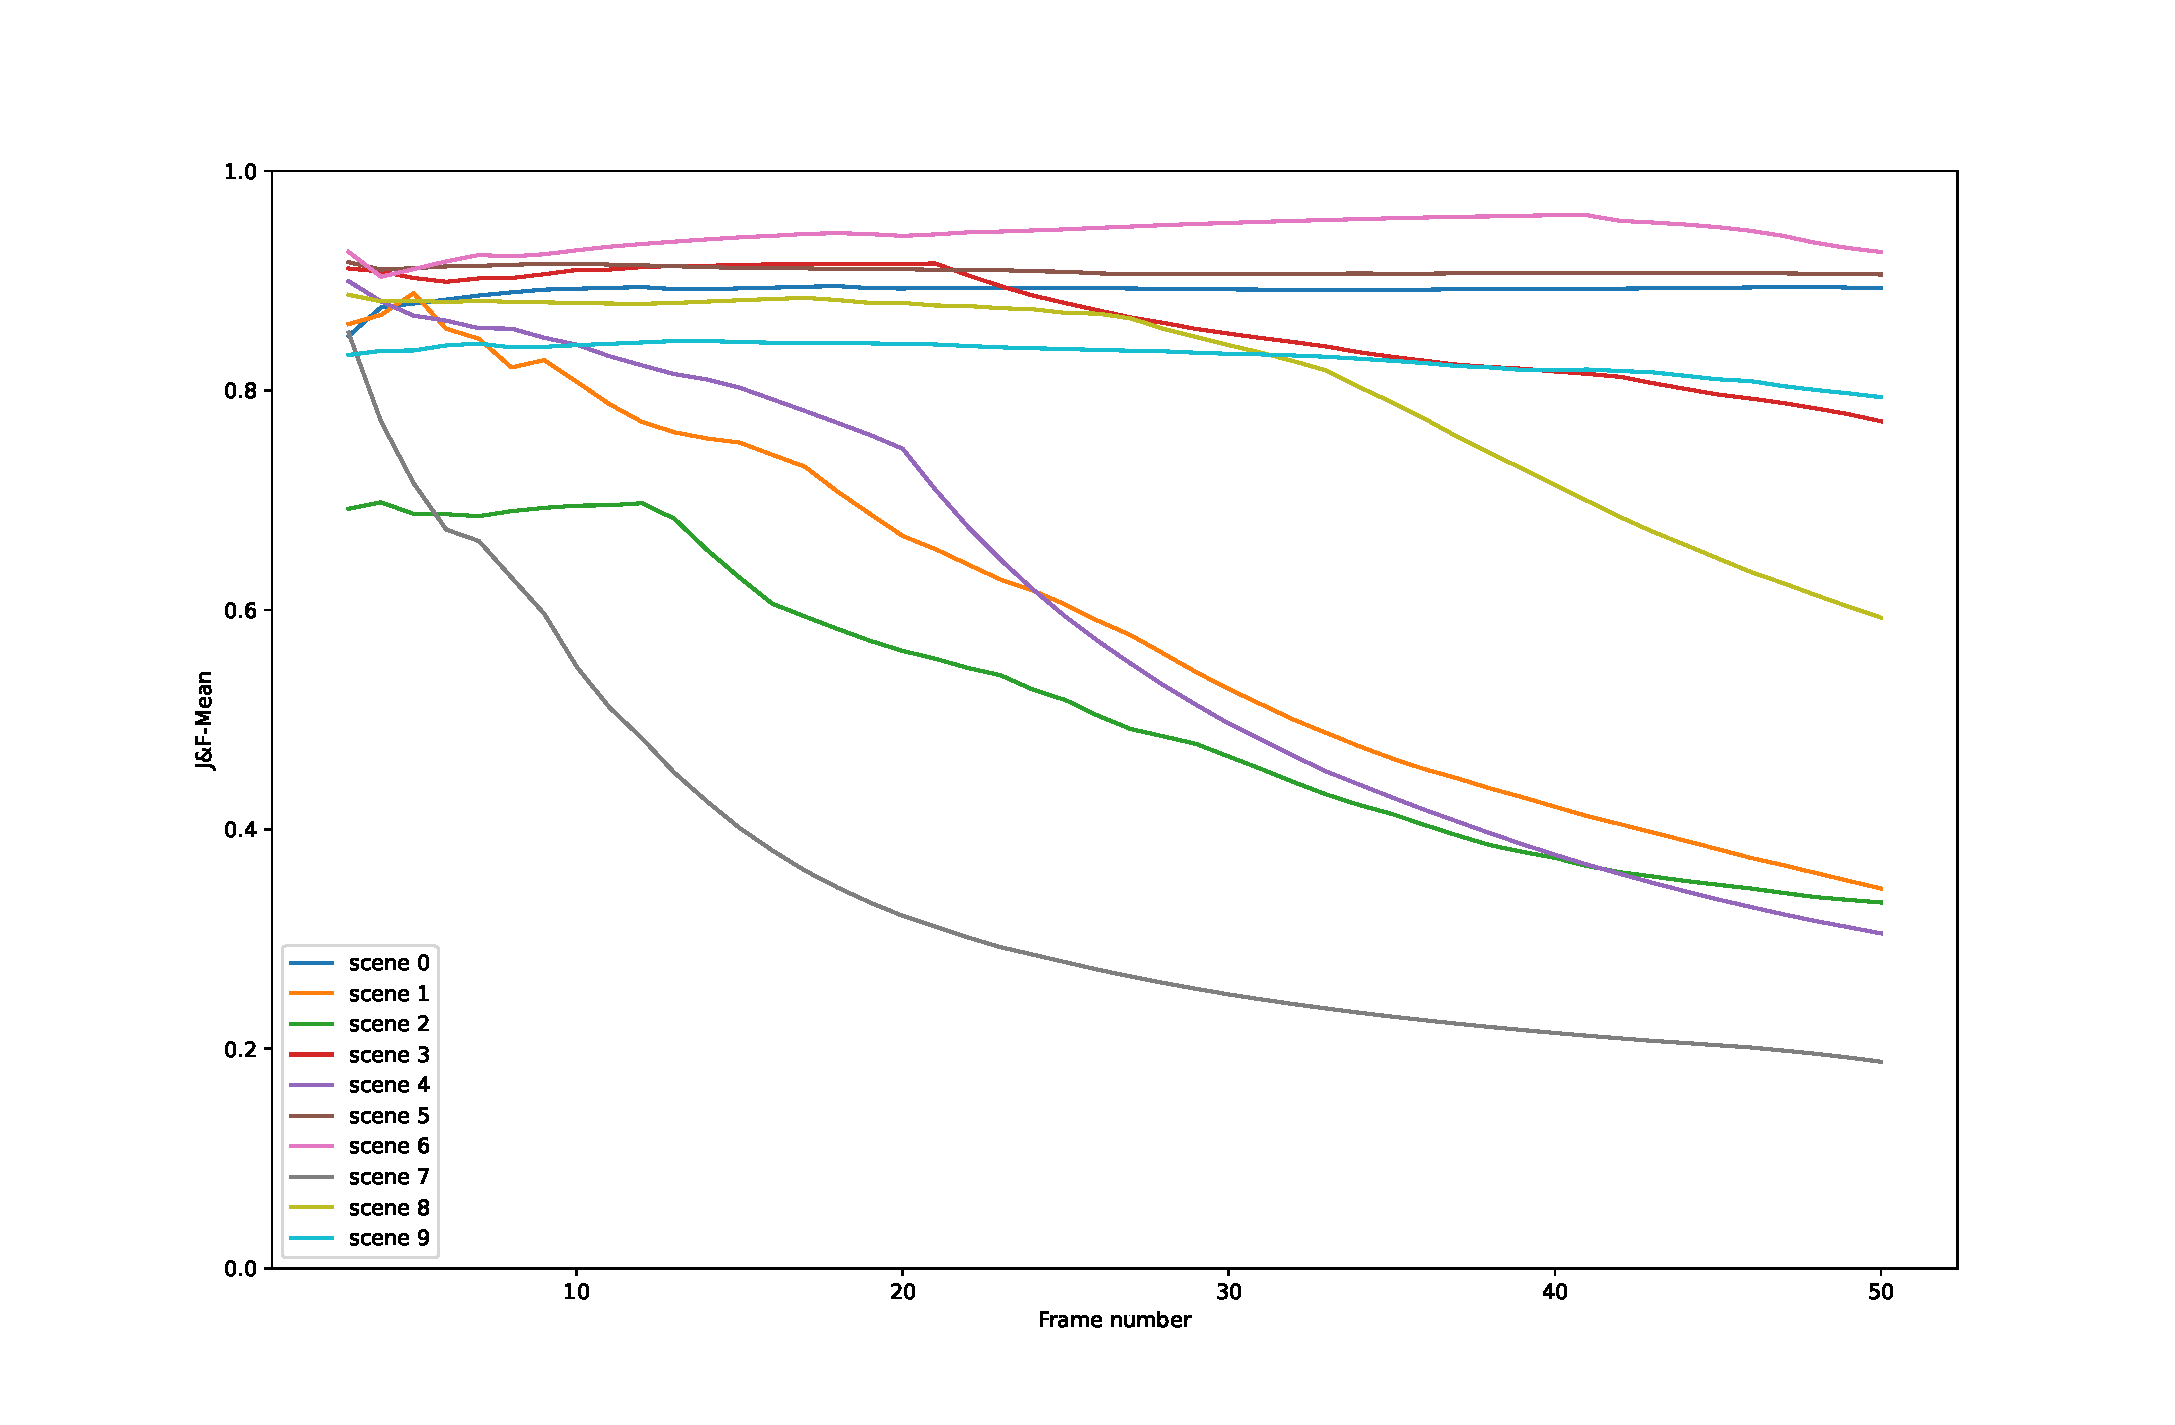
\includegraphics[trim={ 0 2cm 0 1.75cm},width=0.6\linewidth]{figures/appendix/5_bbox_att_fpn_fast_rotation-J_F.pdf}
    \caption{J\&F-Mean bounding box encoder on all rotation fast sequences}
    \label{fig:bbox_j_f}
    
\end{figure}

\begin{figure} [ht!]
    \centering
    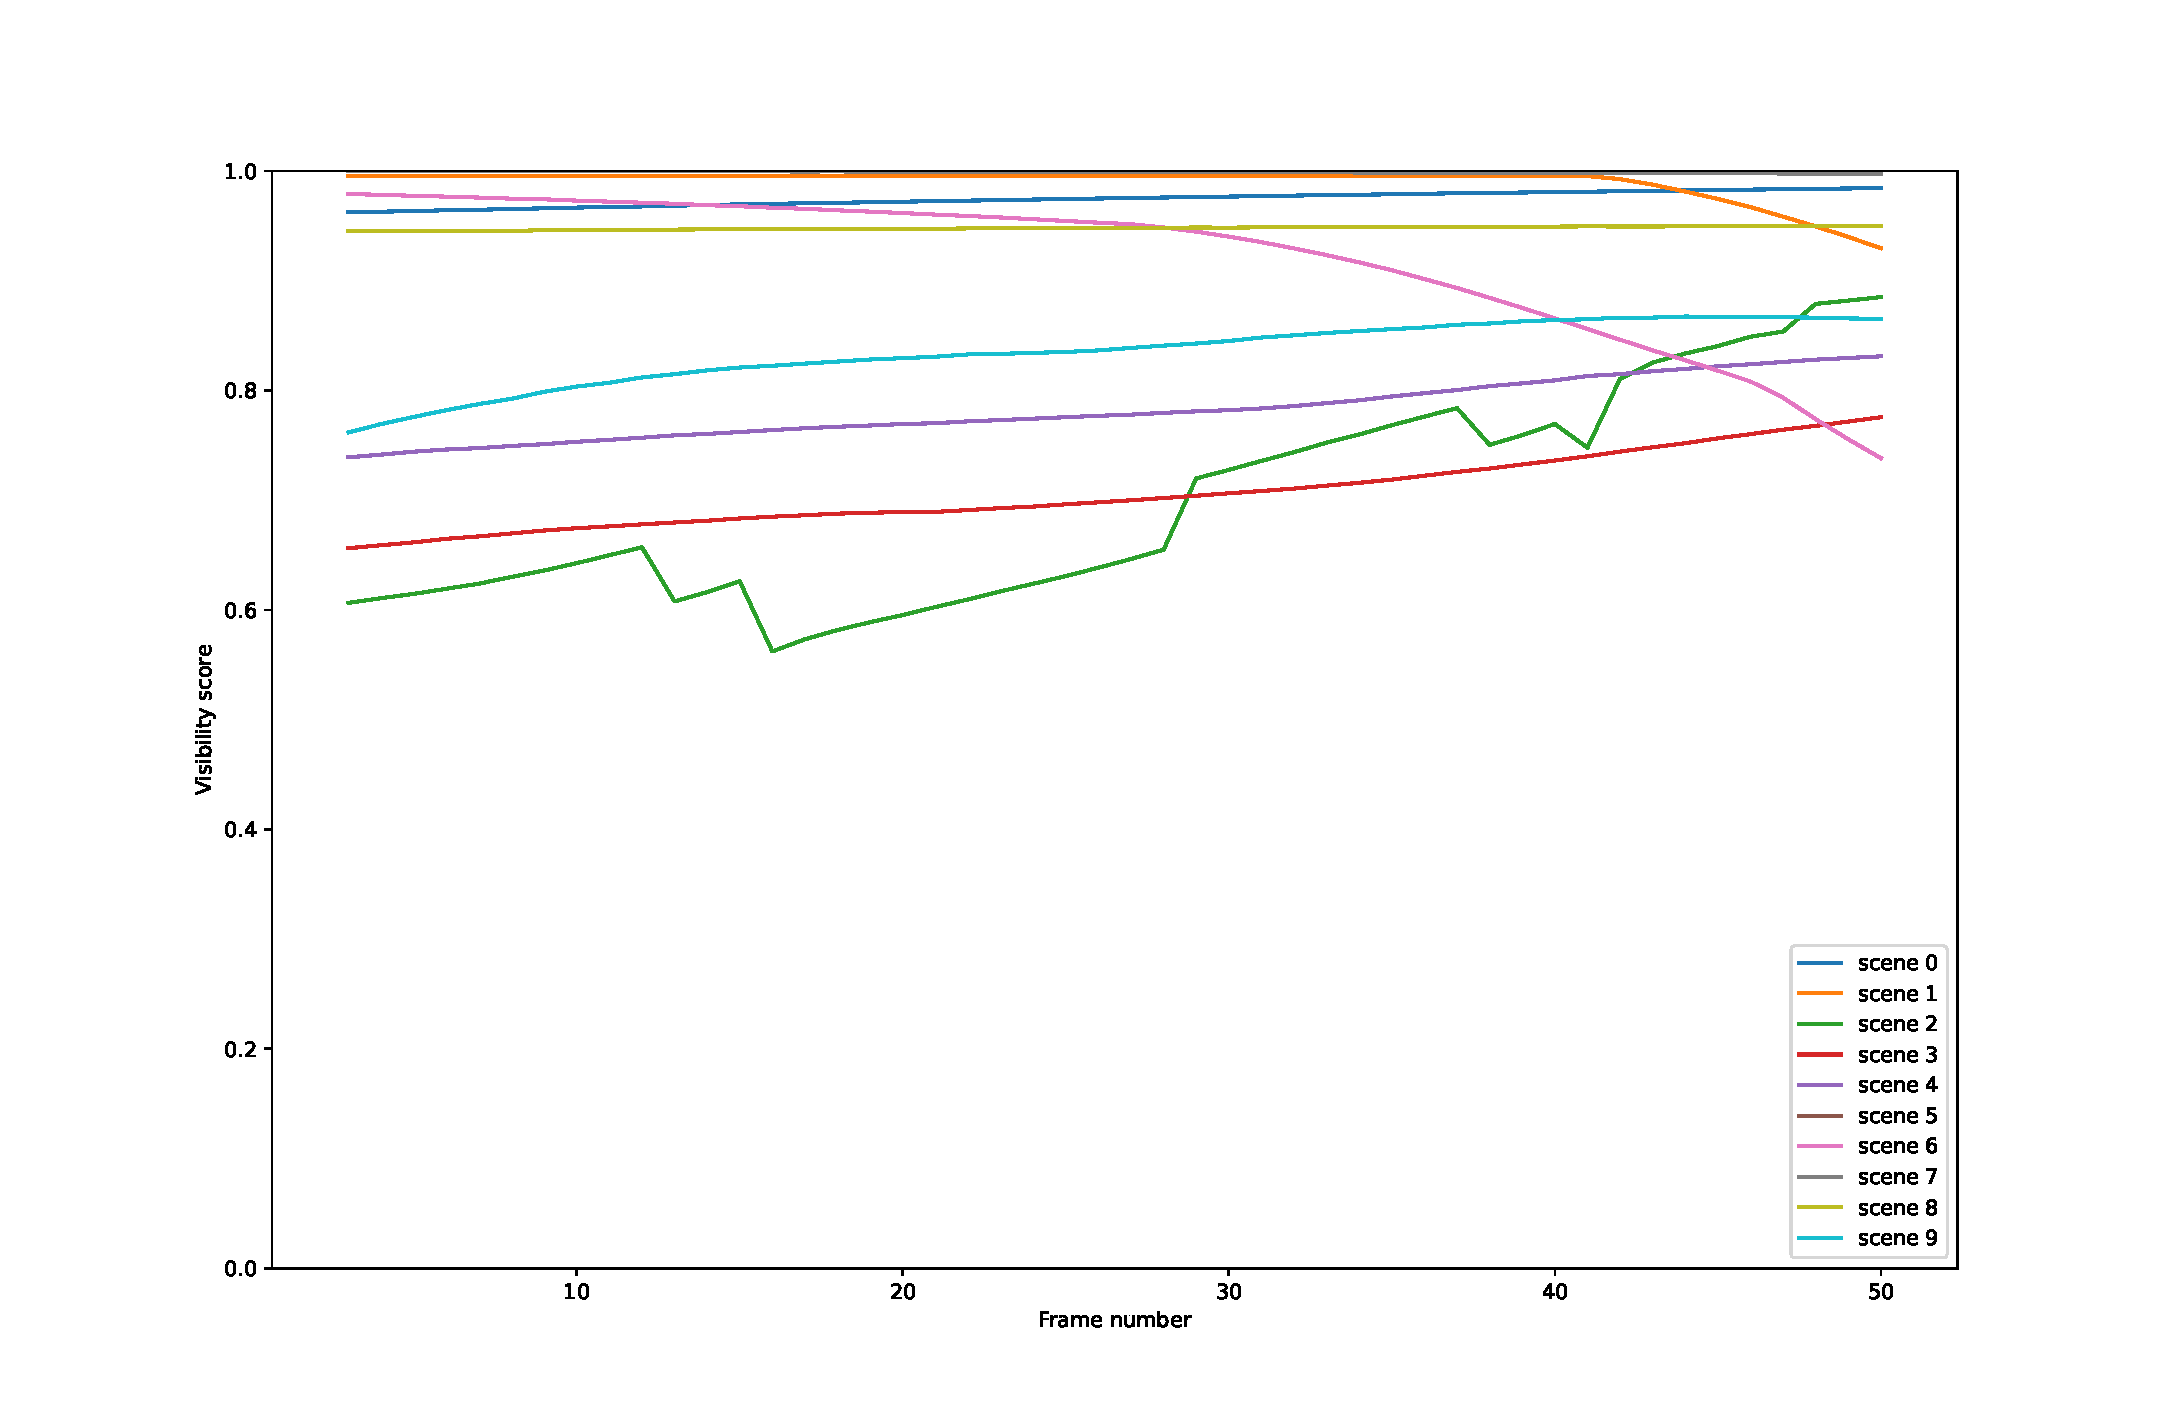
\includegraphics[trim={ 0 2cm 0 2.5cm},width=0.6\linewidth]{figures/appendix/5_bbox_att_fpn_fast_rotation-visibility.pdf}
    \caption{Visibility score bounding box encoder on all rotation fast sequences}
    \label{fig:bbox_visibility}
    
\end{figure}
\begin{figure} [ht!]
    \centering
    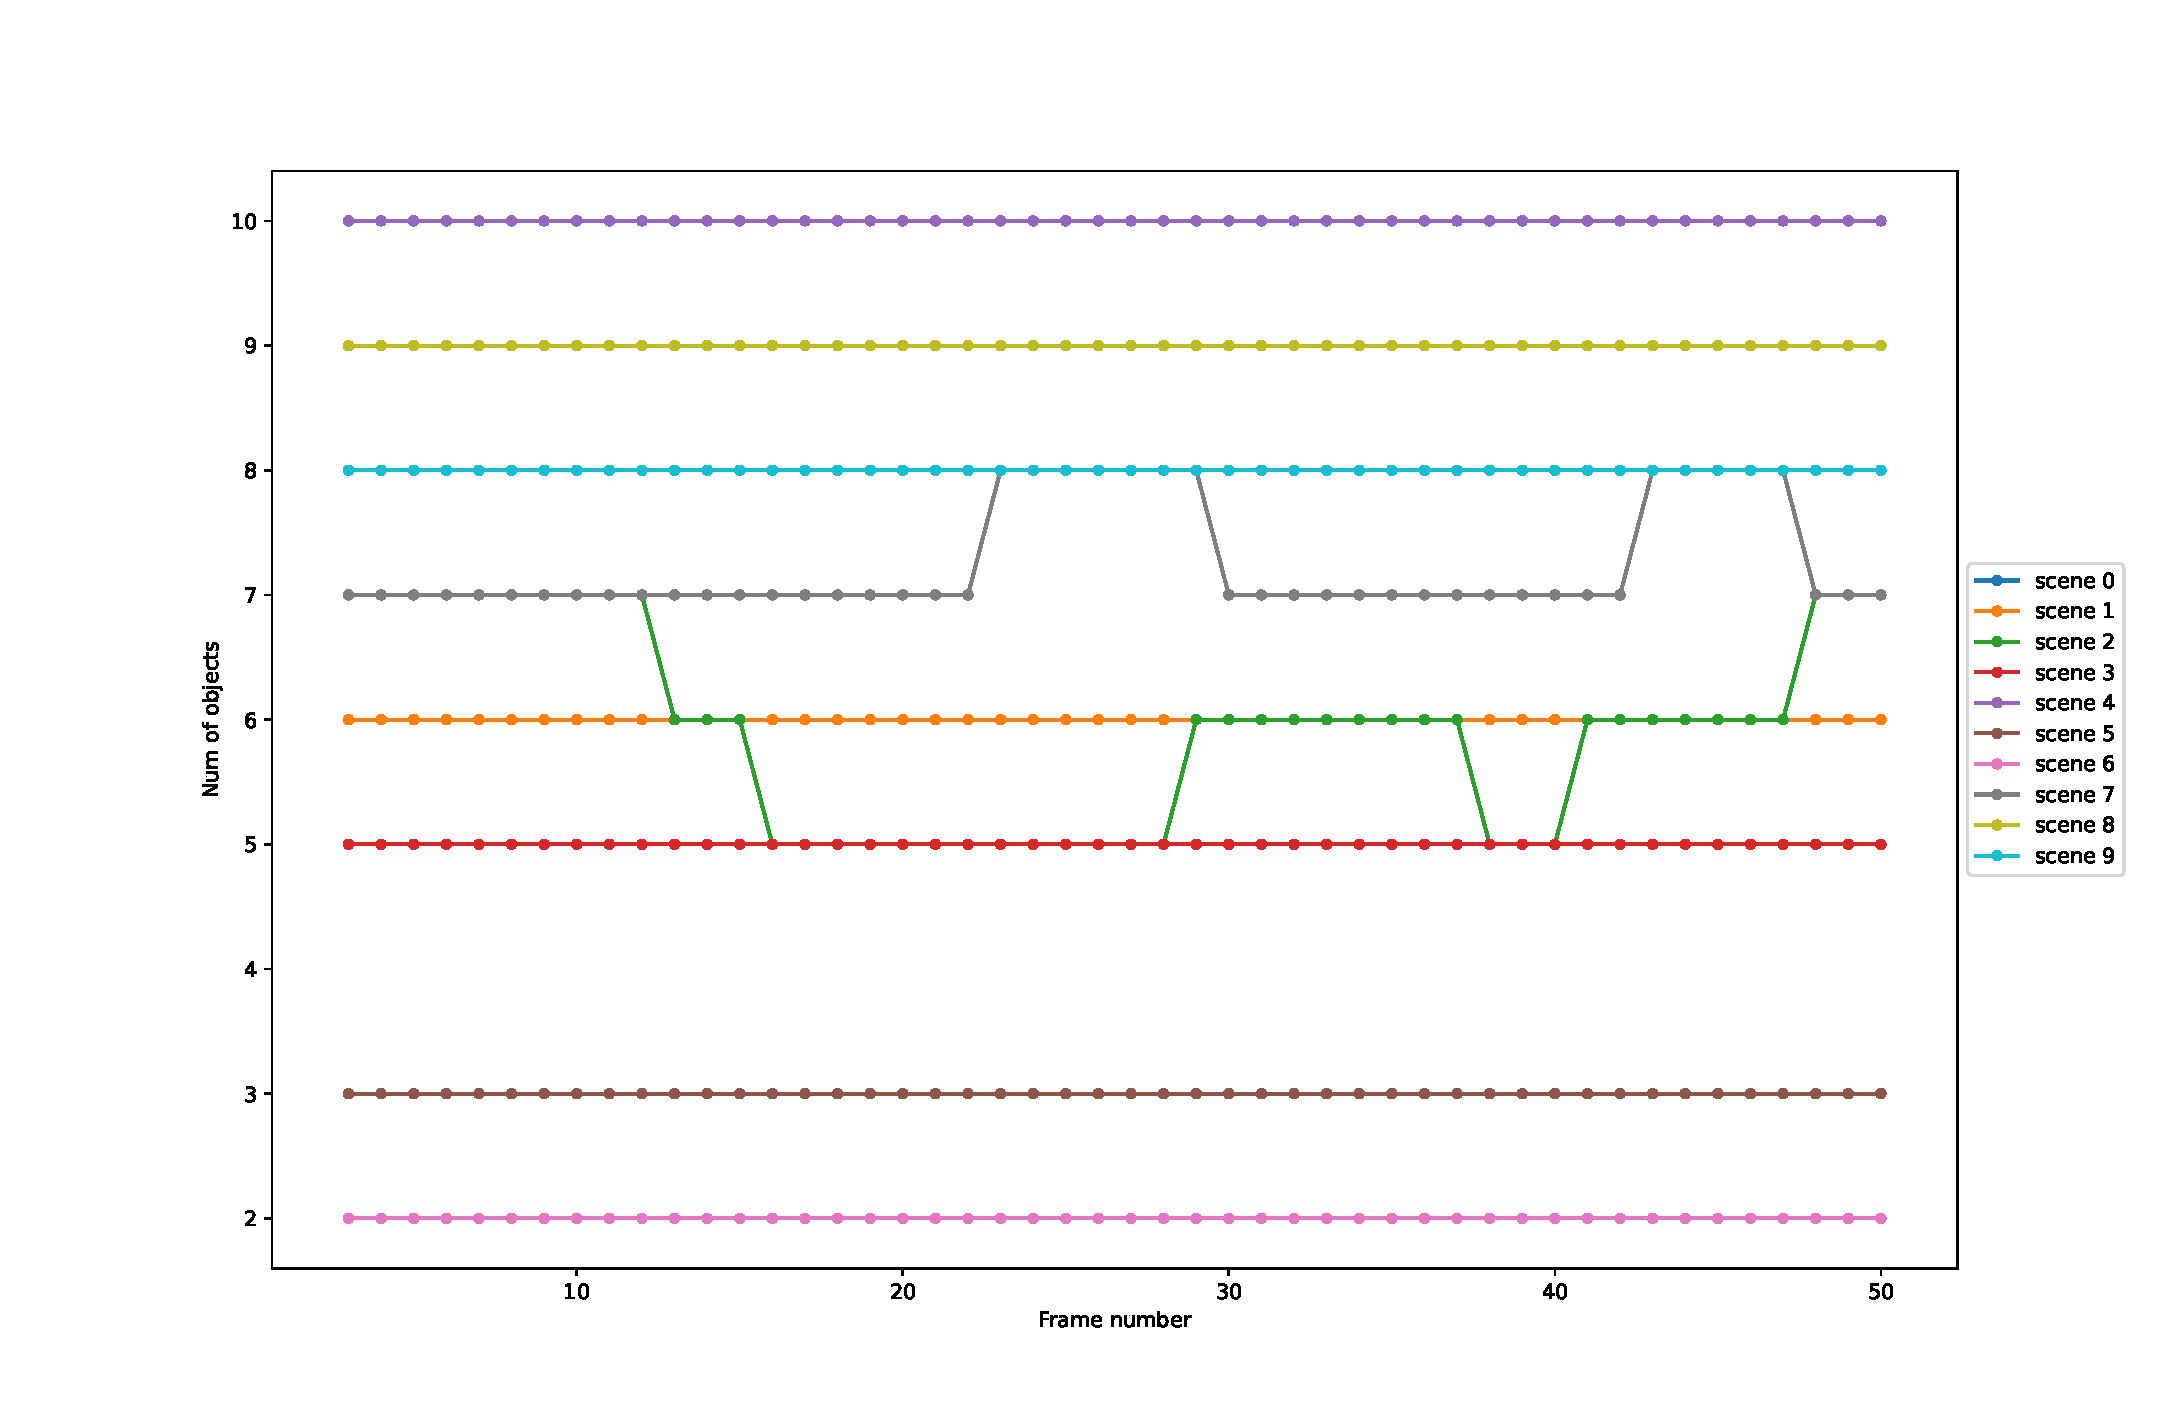
\includegraphics[trim={ 0 2cm 0 2.5cm},width=0.6\linewidth]{figures/appendix/5_bbox_att_fpn_fast_rotation-crowdness.pdf}
    \caption{Num. of objects bounding box encoder on all rotation fast sequences}
    \label{fig:bbox_crowdness}
    
\end{figure}
%%%%%%%%%%%%%%%% mask %%%%%%%%%%%%%%%%%%%%%%%%%%%%%%%%

\begin{figure} [ht!]
    \centering
    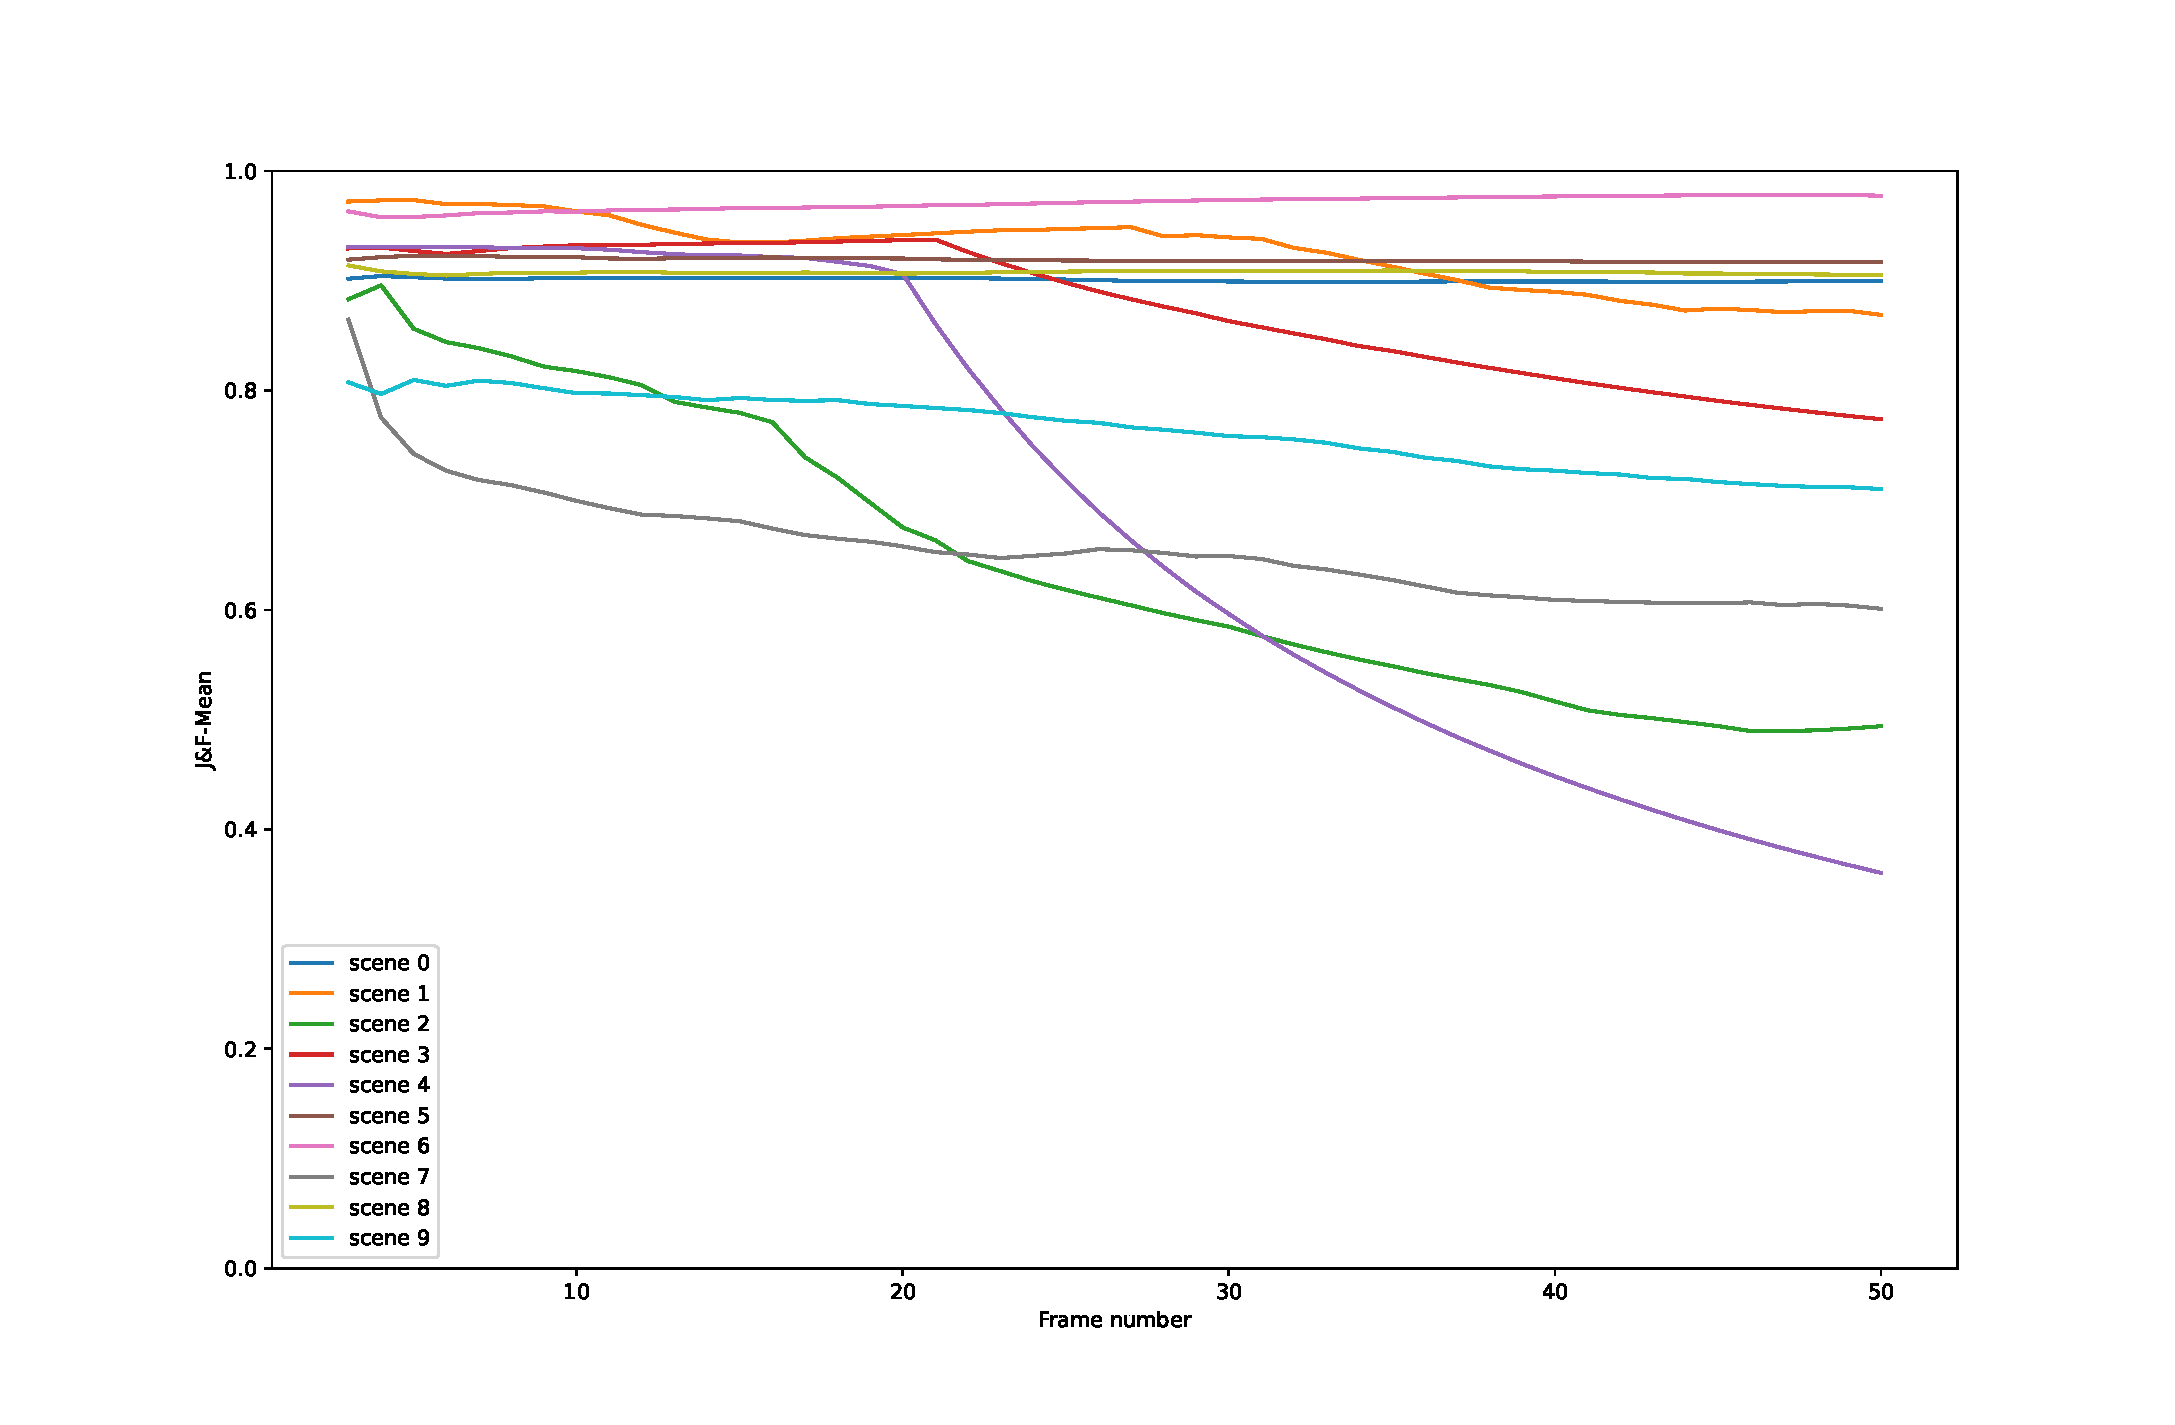
\includegraphics[trim={ 0 2cm 0 1.75cm},width=0.6\linewidth]{figures/appendix/6_mask_att_fpn_fast_rotation-J_F.pdf}
    \caption{J\&F-Mean mask encoder on all rotation fast sequences}
    \label{fig:mask_j_f}
    
\end{figure}

\begin{figure} [ht!]
    \centering
    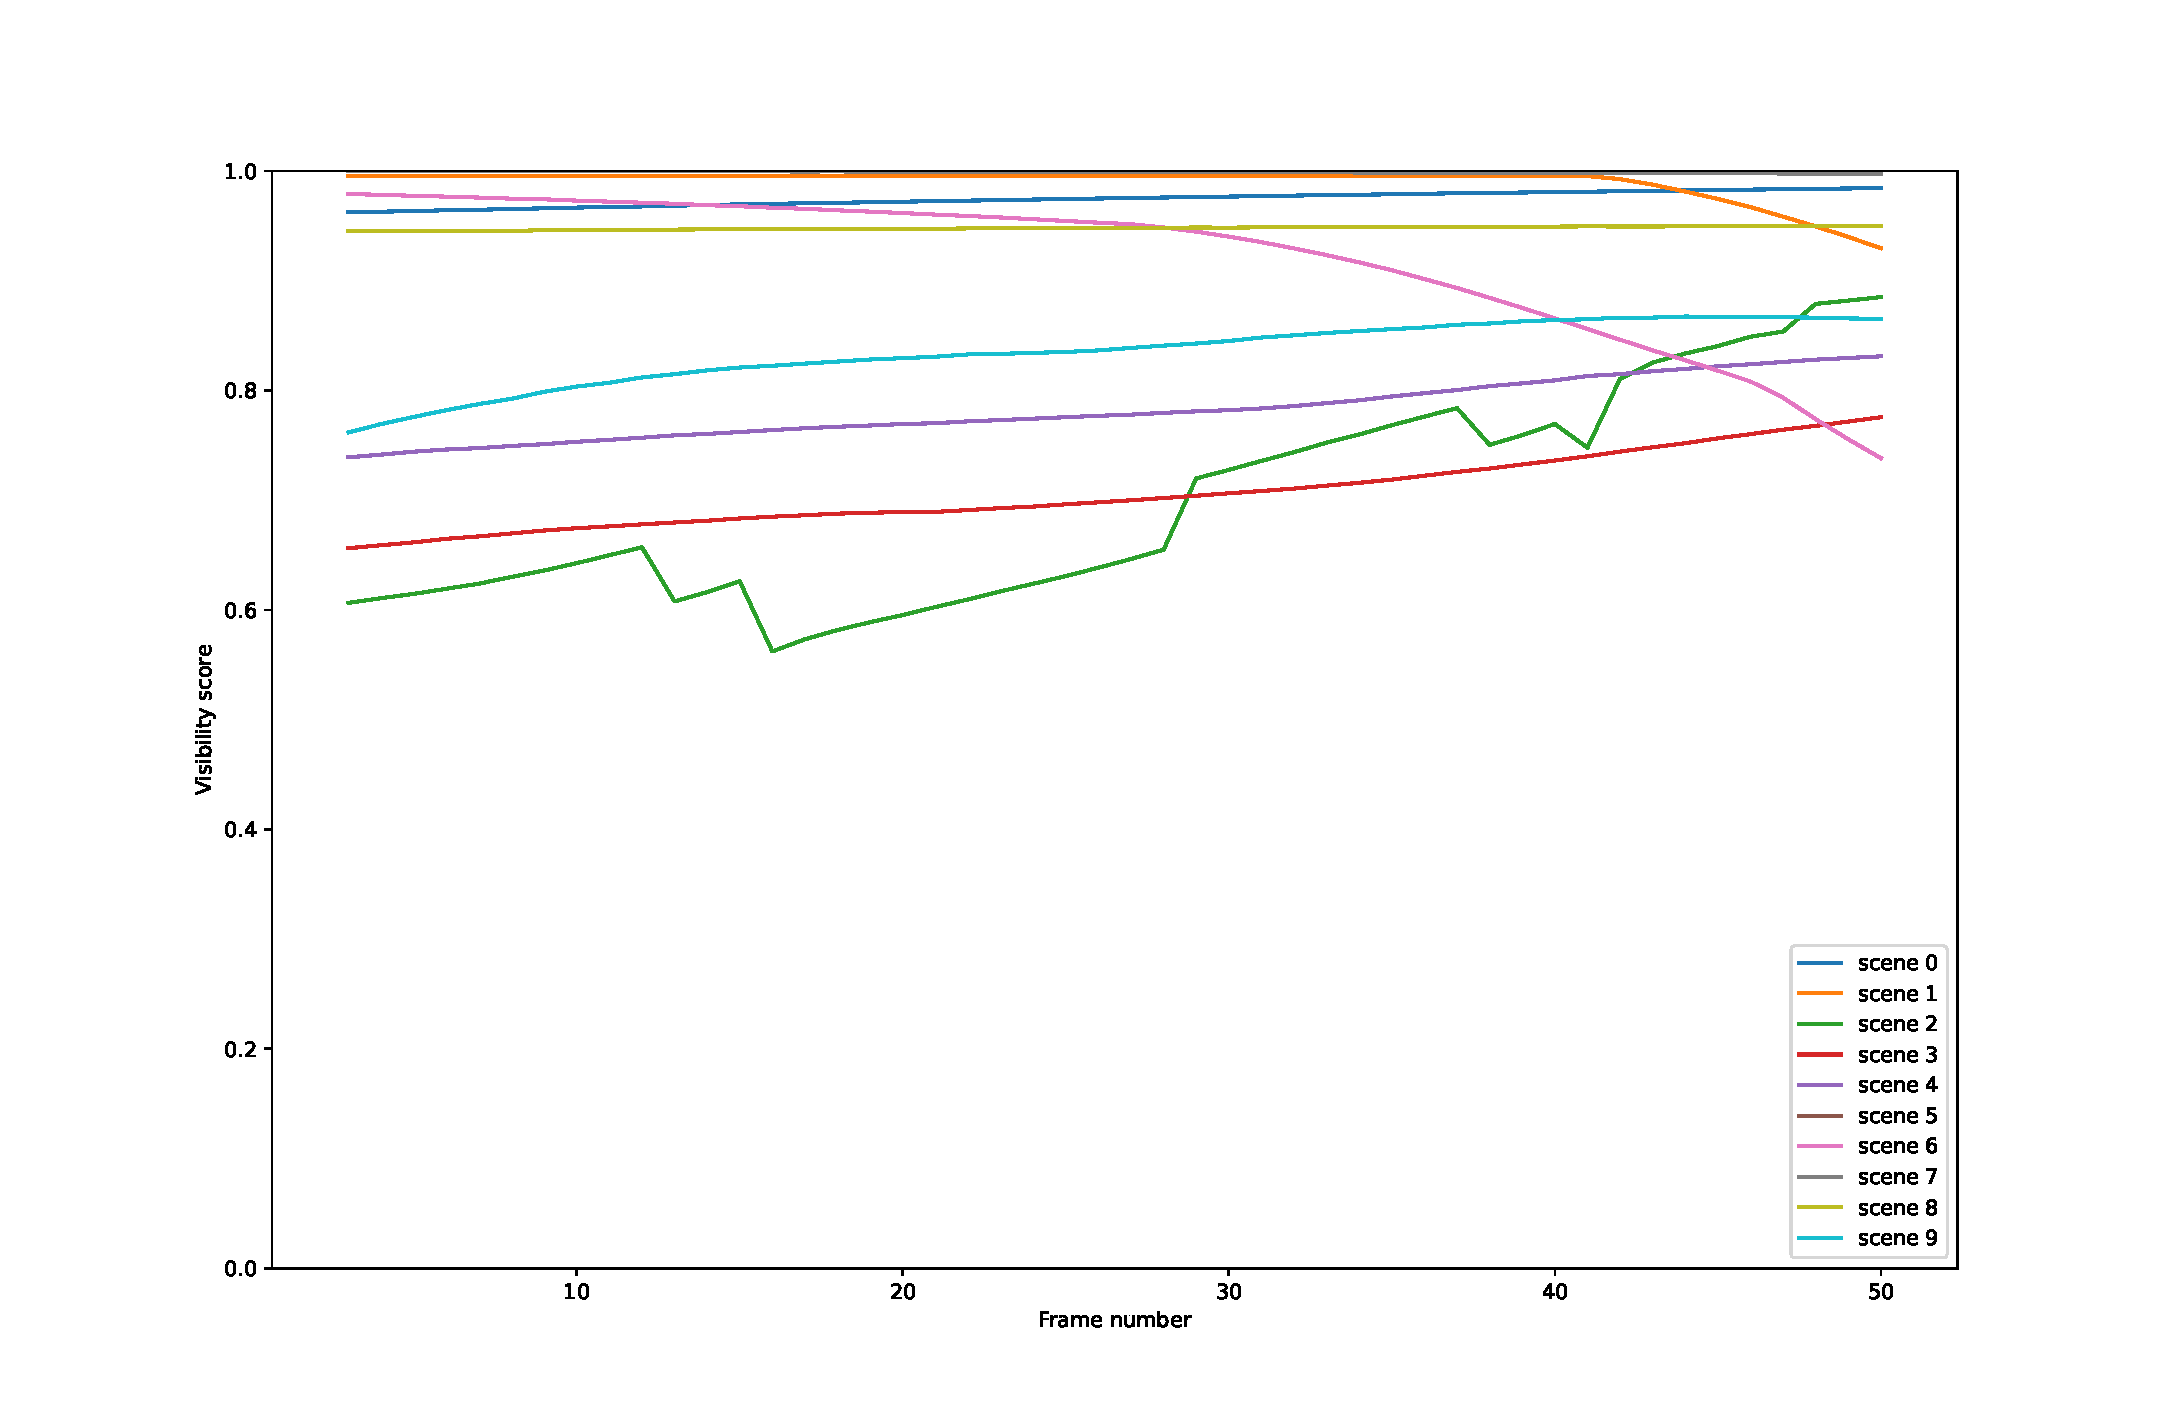
\includegraphics[trim={ 0 2cm 0 2.5cm},width=0.6\linewidth]{figures/appendix/6_mask_att_fpn_fast_rotation-visibility.pdf}
    \caption{Visibility score mask encoder on all rotation fast sequences}
    \label{fig:mask_visibility}
    
\end{figure}
\begin{figure} [ht!]
    \centering
    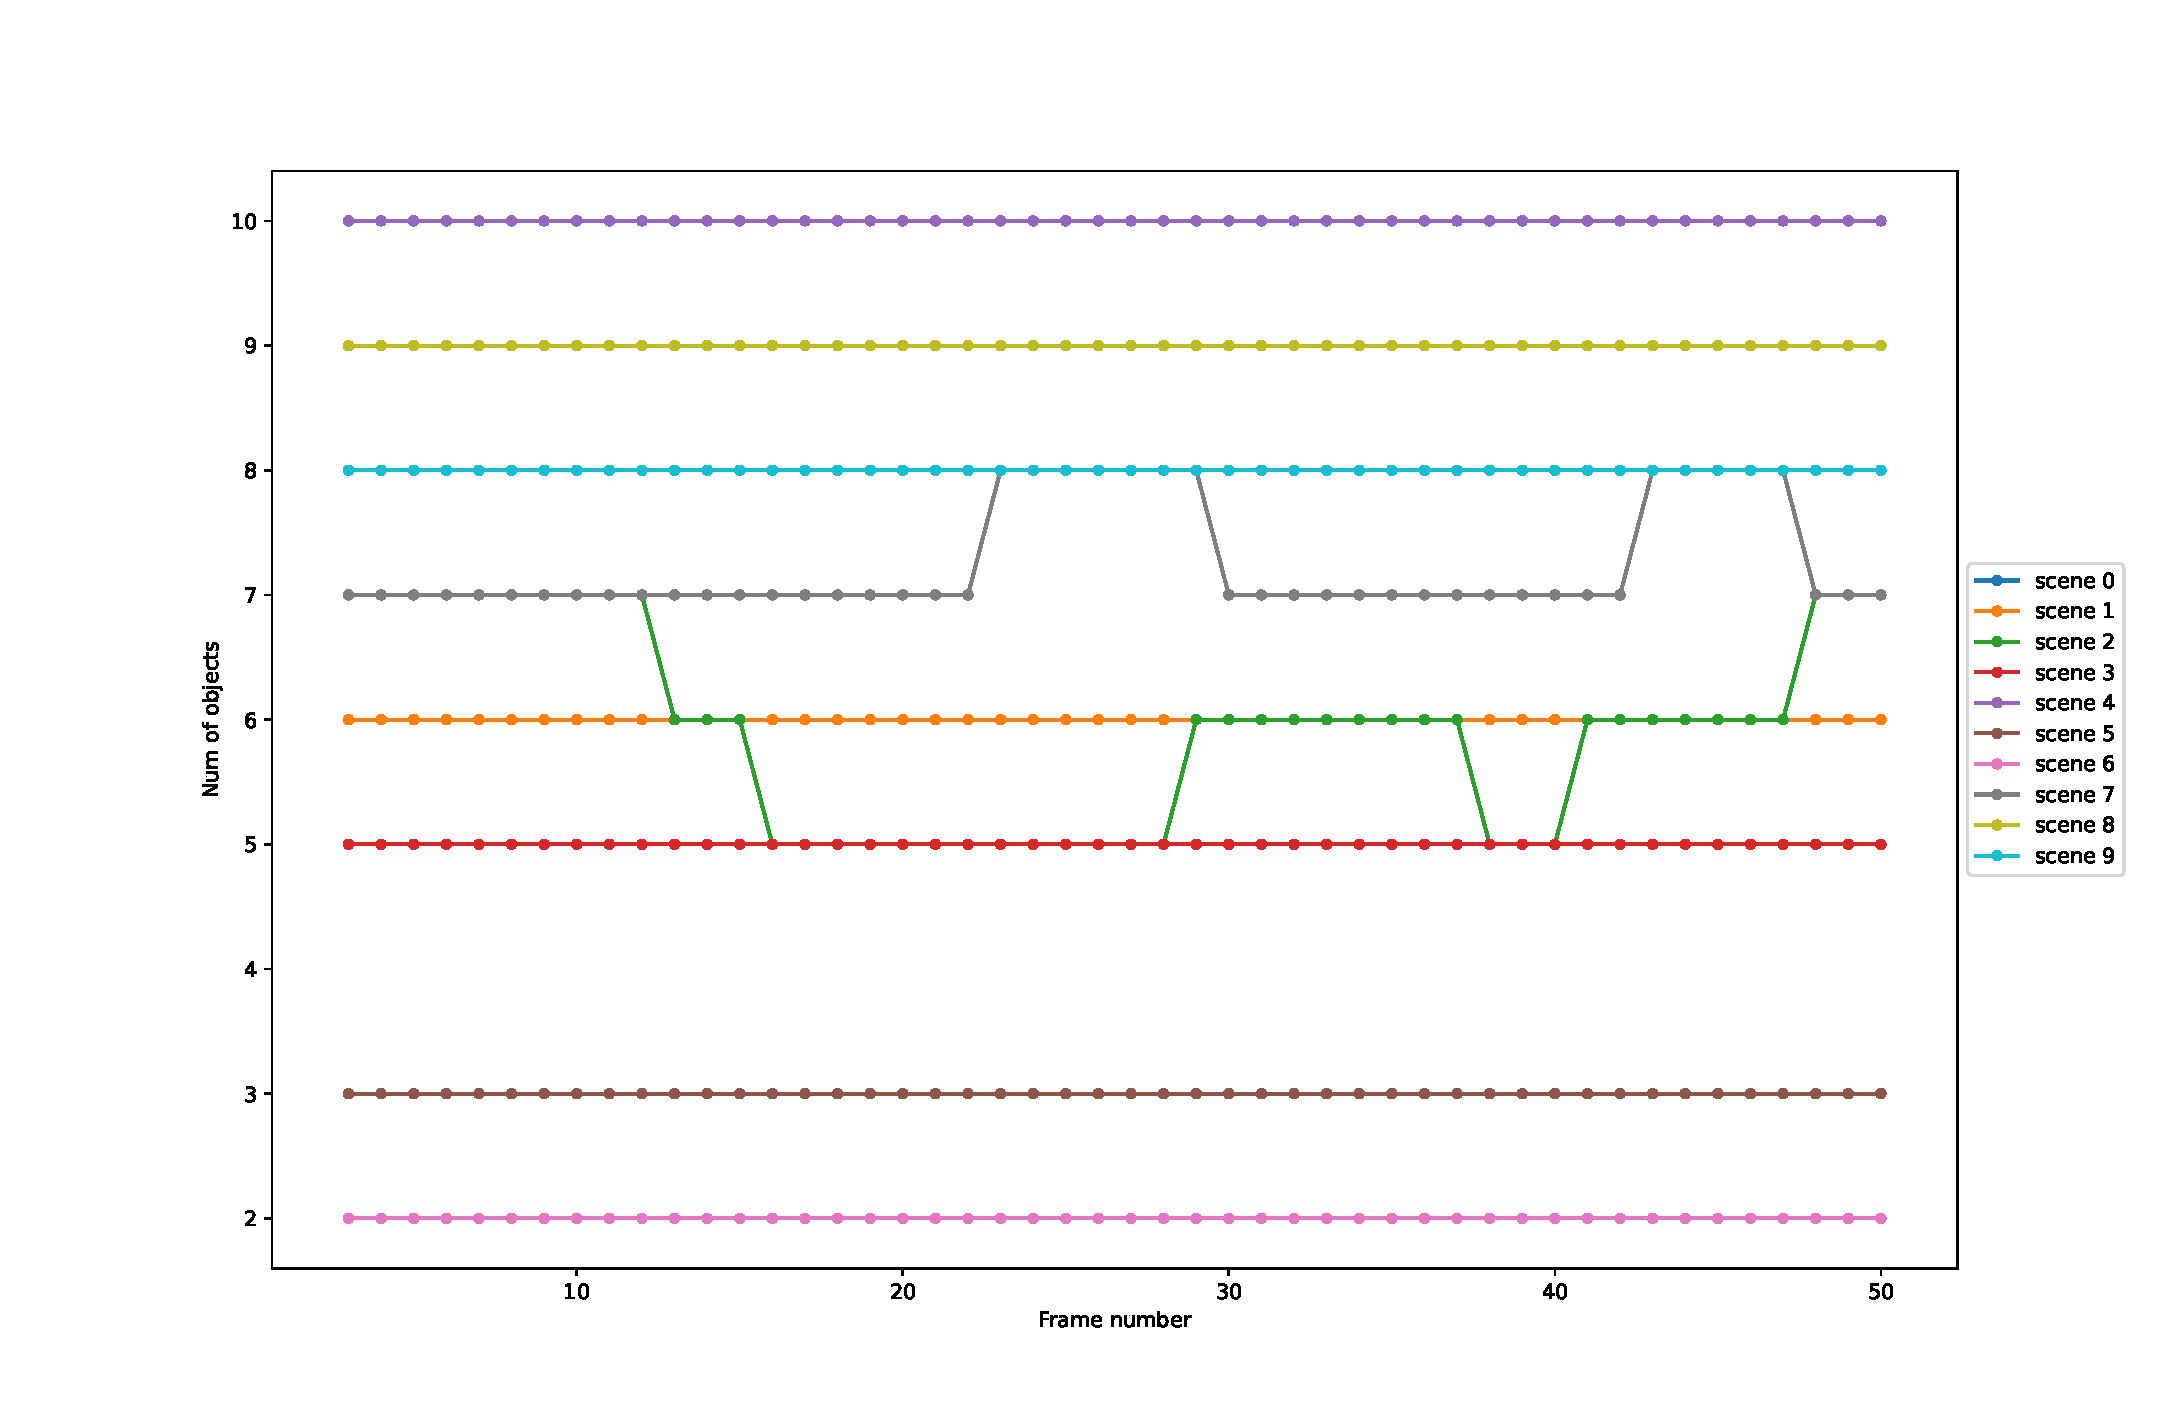
\includegraphics[trim={ 0 2cm 0 2.5cm},width=0.6\linewidth]{figures/appendix/6_mask_att_fpn_fast_rotation-crowdness.pdf}
    \caption{Num. of objects mask encoder on all rotation fast sequences}
    \label{fig:mask_crowdness}
    
\end{figure}
